% Generated from tex/chapters/ch04/08_構築技術.tex for the SWEBOK structure tree
\subsubsection{分散およびクラウド基盤ソフトウェアの構築方法}

分散システムは、物理的に離れた複数の計算機がネットワークで接続され、利用者に一体の資源や機能を提供するシステムである。分散ソフトウェアの構築では、並列性、通信、遅延、部分故障、整合性、セキュリティが問題になる。

分散プログラミングには、クライアントサーバ、三層アーキテクチャ、多層アーキテクチャ、分散オブジェクト、疎結合、密結合などの形がある。

クラウド基盤ソフトウェアでは、マイクロサービス、コンテナ、API ゲートウェイ、サービス登録と発見、監視、自動スケーリングなどを考慮する。従来の分散トランザクションでは ACID 特性を重視することが多い。一方、マイクロサービスでは、すべてを強い整合性で統一するのが難しく、SAGA などによる結果整合性を使うことがある。

\begin{figure}[htbp]
\centering
\IfFileExists{assets/fig-ch04-12.png}{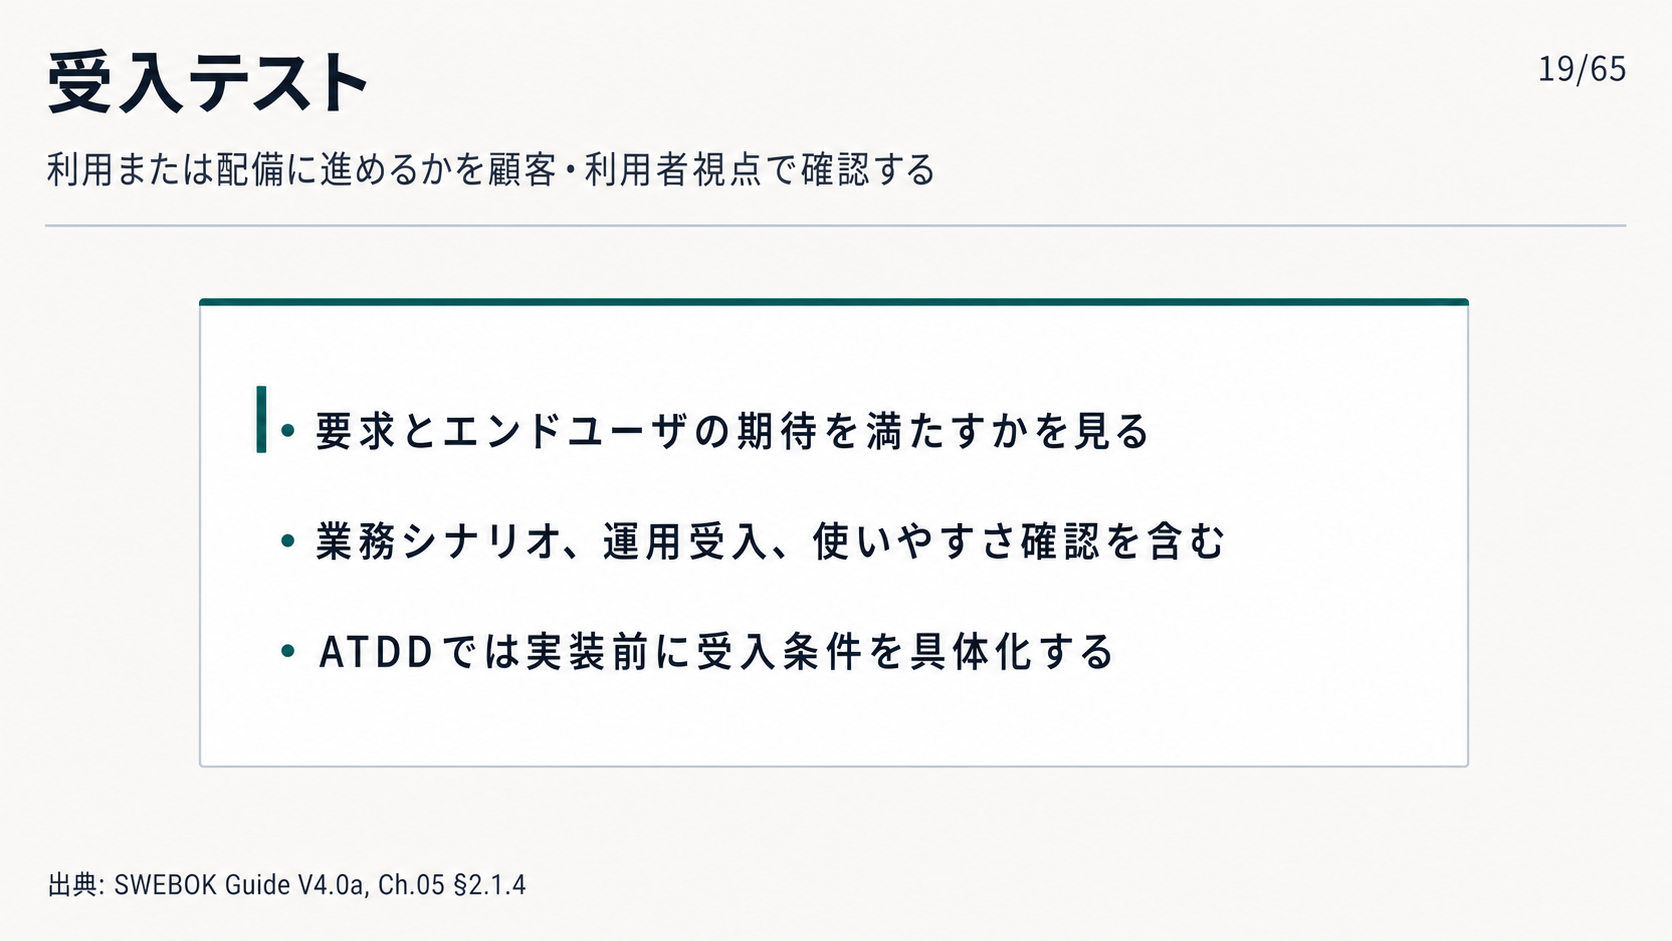
\includegraphics[width=0.96\linewidth]{assets/fig-ch04-12.png}}{\fbox{\parbox[c][48mm][c]{0.9\linewidth}{\centering 画像生成待ち\\分散・クラウド構築の概念図}}}
\caption{分散・クラウド構築の概念図}
\label{fig:ch04-12}
\end{figure}
